\documentclass{article}
\usepackage[utf8]{inputenc}
\usepackage[left=3.5cm, right=3.5cm, top=2.8cm]{geometry}
\usepackage{fancyhdr}
\usepackage{tabularx}
\usepackage{glossaries}
\usepackage{graphicx}
\usepackage{textcomp}
\usepackage{multirow}
\usepackage{caption}
\usepackage{float}
\usepackage{dirtytalk}
\usepackage{hyperref}
\usepackage{listings}
\usepackage[table, x11names]{xcolor}
\usepackage[dvipsnames]{xcolor}
\usepackage[T1]{fontenc}
\usepackage[backend=biber,style=authoryear]{biblatex}
\usepackage[bottom]{footmisc}

\addbibresource{bib.bib}
\setlength\bibitemsep{1.5\itemsep}


\setlength{\extrarowheight}{8pt}

\definecolor{codegray}{rgb}{0.5,0.5,0.5}
\definecolor{backcolour}{rgb}{0.95,0.95,0.92}
\definecolor{codegreen}{rgb}{0,0.6,0}
\definecolor{cadetblue}{rgb}{0.37, 0.62, 0.63}

\lstdefinestyle{mystyle}{
    backgroundcolor=\color{backcolour},   
    commentstyle=\color{codegreen},
    keywordstyle=\color{cadetblue},
    numberstyle=\tiny\color{codegray},
    stringstyle=\color{Cerulean},
    basicstyle=\ttfamily\footnotesize,
    breakatwhitespace=false,         
    breaklines=true,                 
    captionpos=b,                    
    keepspaces=true,                 
    numbers=left,                    
    numbersep=5pt,                  
    showspaces=false,                
    showstringspaces=false,
    showtabs=false,                  
    tabsize=2
}
\newcommand\YAMLcolonstyle{\color{red}\mdseries}
\newcommand\YAMLkeystyle{\color{black}\bfseries}
\newcommand\YAMLvaluestyle{\color{blue}\mdseries}

\makeatletter
\newcommand\language@yaml{yaml}
\expandafter\expandafter\expandafter\lstdefinelanguage
\expandafter{\language@yaml}
{
  keywords={true,false,null,y,n},
  keywordstyle=\color{darkgray}\bfseries\footnotesize,
  basicstyle=\YAMLkeystyle\footnotesize,                                 % assuming a key comes first
  sensitive=false,
  comment=[l]{\#},
  morecomment=[s]{/*}{*/},
  commentstyle=\color{purple}\ttfamily\footnotesize,
  stringstyle=\YAMLvaluestyle\ttfamily\footnotesize,
  moredelim=[l][\color{orange}]{\&},
  moredelim=[l][\color{magenta}]{*},
  moredelim=**[il][\YAMLcolonstyle{:}\YAMLvaluestyle]{:},   % switch to value style at :
  morestring=[b]',
  morestring=[b]",
  literate =    {---}{{\ProcessThreeDashes}}3
                {>}{{\textcolor{red}\textgreater}}1     
                {|}{{\textcolor{red}\textbar}}1 
                {\ -\ }{{\mdseries\ -\ }}3,
}
\newcommand\ProcessThreeDashes{\llap{\color{cyan}\mdseries-{-}-}}
% switch to key style at EOL
\lst@AddToHook{EveryLine}{\ifx\lst@language\language@yaml\YAMLkeystyle\fi}
\makeatother

\lstdefinestyle{ascii-tree}{
    backgroundcolor=\color{backcolour},   
    commentstyle=\color{codegreen},
    keywordstyle=\color{cadetblue},
    numberstyle=\tiny\color{codegray},
    stringstyle=\color{Cerulean},
    basicstyle=\ttfamily\footnotesize,
    breakatwhitespace=false,         
    breaklines=true,                 
    captionpos=b,                    
    keepspaces=true,                 
    numbers=left,                    
    numbersep=5pt,                  
    showspaces=false,                
    showstringspaces=false,
    showtabs=false,                  
    tabsize=2,
    literate={├}{|}1 {─}{--}1 {└}{+}1 
}
  
\lstset{
  style=mystyle,
}

%% FOR QUOTING %%
\def\signed #1{{\leavevmode\unskip\nobreak\hfil\penalty50\hskip2em
  \hbox{}\nobreak\hfil(#1)%
  \parfillskip=0pt \finalhyphendemerits=0 \endgraf}}

\newsavebox\mybox
\newenvironment{aquote}[1]
  {\savebox\mybox{#1}\begin{quote}}
  {\signed{\usebox\mybox}\end{quote}}
%% - %%


\pagestyle{fancy}
\usepackage{graphicx}
\graphicspath{{images/}}
\title{\textbf{DevOps : Continuous Integration and Continuous Deployment applied}
\vspace{10px}\LARGE \\~\\A Degree Thesis\\Submitted to the Faculty of the\\
Escola Tècnica d'Enginyeria de Telecomunicació de Barcelona\\
\vspace{10px} \textbf{Universitat Politècnica de Catalunya}\\
\vspace{10px}by\\
Héctor Pascual Haba\\~\\
\vspace{15px}In partial fulfilment 
of the requirements for the degree in
TELECOMMUNICATION TECHNOLOGIES AND SERVICES ENGINEERING
\\
\vspace{80px}\textbf{Advisor: Israel Martín}
\vspace{30px}\\ Barcelona, June 2020

}

\rhead{
\includegraphics[width=2cm]{etsetb.png}}
\lhead{
\includegraphics[width=4cm]{upc.png}}
\setlength\headheight{26pt} 
\renewcommand{\headrulewidth}{0pt}

% Redefine the plain page style
\fancypagestyle{plain}{%
    \fancyhf{}%
    \fancyfoot[R]{\thepage}%
    \rhead{
\includegraphics[width=2cm]{etsetb.png}}
    \lhead{
\includegraphics[width=4cm]{upc.png}}
    \setlength\headheight{26pt} 
    \renewcommand{\headrulewidth}{0pt}
}

\date{}
\makeglossaries
\newglossaryentry{CI}
{
    name=CI,
    description={Acronym for continuous integration, a software practice which consists in making automatic continuous integration of a project}
}
\newglossaryentry{TDD}{
    name=TDD,
    description={Acronym for test driven development, consists on creating tests from a developer’s perspective and write code in order to make tests work}
}
\newglossaryentry{CD}
{
    name=CD,
    description={Acronym for continuous deployment, a software practice which consists in making automatic continuous deployments of a project}
}
\newglossaryentry{RDBMS}
{
    name=RDBMS,
    description={Acronym for Relational Database Management System}
}
\newglossaryentry{DSL}{
    name=DSL,
    description={Acronym for Domain Specific Language, a language specialized only for an application domain}
}
\newglossaryentry{SW}{
    name=SW,
    description={Acronym for Software}
}
\newglossaryentry{IaC}{
    name=IaC,
    description={Acronym for Infrastructure as Code, process of managing infrastructure through definition files}
}
\newglossaryentry{VCS}{
    name=VCS,
    description={Acronym for Version Control System}
}
\newglossaryentry{API}{
    name=API,
    description={Acronym for Application Programming Interface}
}
\newglossaryentry{WSGI}{
    name=WSGI,
    description={Acronym for Web Server Gateway Interface, a calling convention for web servers to forward requests to web applications}
}
\newglossaryentry{SSH}{
    name=SSH,
    description={Acronym for Secure Shell, a protocol for accessing machines remotely}
}
\newglossaryentry{SQL}{
    name=SQL,
    description={Acronym for Structured Query Language, a domain specific language for managing relational database systems}
}

\begin{document}
\maketitle
\pagenumbering{gobble}

\clearpage
\setcounter{page}{1}
\pagenumbering{arabic}
\addcontentsline{toc}{section}{Abstract}
\section*{Abstract}
\large	
DevOps is a trending concept in the \gls{SW} industry introduced and popularized during the last decade, this thesis goes deep into the concept, the culture and fields related to it which are present in almost each project and company nowadays. The research model followed in the thesis basically consists in getting in contact with the DevOps culture by designing, developing and implementing a Python tool with some Continuous Integration and Continuous Deployment features. Basically this tool consists on a back-end REST API capable of creating and automating builds on any connected slave node to the tool, similar to traditional DevOps tools logic such as Jenkins or TeamCity, but in a lightweight, portable and OS independent solution, also a front-end is developed in order to make the tool easier and simpler to use. In order to demonstrate the power and the capabilities of the tool we will containerize a build environment with Docker and automate its build process with the tool as well as deploying the binaries resulting from the build process.

\newpage
\addcontentsline{toc}{section}{Resum}
\section*{Resum}
DevOps es un concepte tendència a la indústria del SW, introduït i popularitzat durant la darrera decada, aquesta tesis aprofundeix en el concepte, la cultura i aspectes relacionats, que son present a la majoria de projectes i empreses avui en dia. El model d'investigació a seguir durant la tesis es basa en entrar en contecte directe amb la cultura de DevOps dissenyant, desenvolupant i implementant una eina en Python amb característiques tant de Integració Continua com de Desplegament Continuu. En resum, la eina consisteix en un backend REST API que permet la creació i automatització de construccions de projectes en qualsevol node esclau conectat a la eina, de manera semblant a eines tradicional de DevOps com son Jenkins o Teamcity pero d'una manera lleugera, portable i independent del sistema operatiu. Tambe s'ha desenvolupat un frontend per facilitar l'us de l'eina. Finalment, per a demostrar el funcionament i la capacitat de l'eina crearem un entorn de construcció amb docker del qual automatitzarem el procés de construcció amb l'eina a més de desplegar els binaris resultants del procés.

\newpage
\addcontentsline{toc}{section}{Resumen}
\section*{Resumen}
DevOps es un concepto de tendencia en la industria del SW introducido y popularizado durante la última década, esta tesis profundiza en el concepto, la cultura y los campos relacionados que están presentes en casi cada proyecto y empresa en la actualidad. El modelo de investigación seguido en la tesis consiste básicamente en ponerse en contacto con la cultura DevOps mediante el diseño, desarrollo e implementación de una herramienta Python con algunas características de integración continua y despliegue continuo. Básicamente, esta herramienta consiste en una API REST de back-end capaz de crear y automatizar compilaciones en cualquier nodo esclavo conectado a la herramienta, similar a la lógica de herramientas DevOps tradicionales como Jenkins o TeamCity, pero en una solución ligera, portátil e independiente del sistema operativo, también un front-end se ha desarrollado para hacer que la herramienta sea más fácil y simple de usar. Para demostrar el poder y las capacidades de la herramienta, contenerizaremos un entorno de compilación con Docker y automatizaremos su proceso de compilación con la herramienta, así como desplegaremos los binarios resultantes del proceso de compilación.

\newpage
\addcontentsline{toc}{section}{Acknowledgments}
\section*{Acknowledgments}
I would first like to thank my thesis advisor Israel Martin of the ETSETB at Politechnics University of Catalonia, due to his instant e-mail answers when I ran into a trouble spot or had a question about my research or writing. He consistently allowed this thesis to be my own work, but guided me in the right the direction whenever he thought I needed it.
\\~

I would also like to thank my supervisor Oscar Alonso from TTTech Auto Iberia, the company I was when this project was carried out, due to his corrections and document validations as well as technical support. Also DevOps department colleagues which were always available for technical issues and give me a hand when I needed it. It is always good to have a technical support when you are entering and discovering a new field on research.
\\~

Finally, I must express my very profound gratitude to my parents for providing me with unfailing support and continuous encouragement throughout my years of study and through the process of researching and writing this thesis. This accomplishment would not have been possible without them. 
\\~

Thank you all who have helped in one way or another to make this project possible.

\newpage
\section*{Revision history and approval record}
\vspace{0.5cm}
\begin{table}[!h]
\begin{tabularx}{\textwidth}{|l|l|X|}
\hline
\textbf{Revision} & \textbf{Date} & \textbf{Purpose} \\ \hline
0                 & 20/04/2020    & Document Creation \\ \hline
1                 & 22/05/2020    & Minor corrections proposed by tutor \\ \hline
2                 & 06/06/2020    & Minor corrections proposed by tutor \\ \hline
3                 & 29/06/2020    & Final version corrections \\ \hline

\end{tabularx}
\caption{Revision history and approval record}
\end{table}
~\\
\begin{table}[!h]
\begin{tabularx}{\textwidth}{|l|X|}
\hline
\textbf{Name} & \textbf{e-mail} \\ \hline
Héctor Pascual & rcpascualhector@gmail.com \\ \hline
Israel Martín & israel.martin@upc.edu \\ \hline
Óscar Alonso &  oscar.alonso@tttech-auto.com \\ \hline
\end{tabularx}
\caption{Document distribution list}
\end{table}
~\\
\begin{table}[!h]
\begin{tabularx}{\textwidth}{|l|l|X|}
\hline
 & \textbf{Written by : } & \textbf{Reviewed and approved by :} \\ \hline
\textbf{Name}                & Hector Pascual    & Oscar Alonso and Israel Martín \\ \hline
\textbf{Position}            & Project Author    & Project Supervisor and Advisor \\ \hline

\end{tabularx}
\caption{Approval Record}
\end{table}
\newpage

\addcontentsline{toc}{section}{Table of Contents}
\tableofcontents
\newpage

\addcontentsline{toc}{section}{List of Figures}
\listoffigures

\newpage
\addcontentsline{toc}{section}{List of Tables}
\listoftables

\newpage
\section{Introduction}

The project is carried out at TTTech Auto Iberia an automotive company which works with embedded projects and big build environments that can be automatized in different ways, during my stay in the company I have got in touch with DevOps related concepts such as automatizing infrastructure deployment, containerizing build environments, designing Continuous Integration pipelines, between other. I have taken all this knowledge learnt and decided to focus my thesis on creating an own \gls{CI} and \gls{CD} tool capable of doing most of the common \gls{CI}/\gls{CD} features such as automatizing builds, taking as input pipeline files, storing artifacts resulting from builds, capability of scheduling jobs through cron expressions and so on.

\subsection{Statement of purpose}

Along this project I will go deep into the DevOps culture and the trending concepts related to it, which are present in almost each project and company nowadays by designing, developing and implementing a Python tool with some \gls{CI} and \gls{CD} features.
\\~\\
The project main goals are:
\begin{itemize}
	\item Get involved with trending DevOps technology.
	\item Get a deep knowledge on DevOps culture and its related concepts.
	\item Develop a \gls{CI} / \gls{CD} (Continuous Integration / Continuous Deployment ) tool with features based on other \gls{CI} tools.
	\item Containerize a build environment and automate its build process as an example.
\end{itemize}


\subsection{Requirements and specifications}

The requirements for the project are strictly related with the tool developed and with the coverage of all DevOps concepts that are connected to the tool implementation. 

\begin{itemize}
	\item The project should cover in deep all the DevOps related concepts mentioned in the sections.
	\item The project should contain reflections on different ways to perform automation of processes.
	\item The development of the tool should be submitted to constant commits to a VCS (git for this project).
	\item The tool should be able to automatize any process that can be done manually via shell commands.
	\item The tool should be able to schedule jobs periodically through cron expressions.
	\item The tool should be able to describe the processes to automatize through pipelines.
	\item The tool should be able to store binary artifacts after a successful build.
\end{itemize}

Referring to the specifications:
\begin{itemize}
	\item The project will contain technical examples when an automation process is described (i.e: Wrapping up a build environment with Docker and deploying it with Ansible to multiple physical hosts.)
	\item The tool will be able to be hosted on any OS system connected to a network.
	\item The tool will be accessible through a REST \gls{API} developed on Python.
	\item The tool will be also accessible through a Front-end which interacts directly with the REST API back-end in order to ease its use.
	\item The Python version used on development will be at least Python 3.6 due to the constant usage of formatted string literals included in version 3.6 (see PEP-498).
\end{itemize}

\subsection{Project Background}

This project is conceived as an abstraction wrap up and continuation of all the work I have been doing in the company during last year and a half and also a deep analysis and practical implementation of concepts related to DevOps culture that I had to learn in order to proceed. With abstracted I mean that no confidential data will be present on any document. The only way I will be using all the work done internally in the company is as base knowledge and start point to develop this project.
\newpage
\subsection{Work plan}
The structure of the project tasks follows the next order :

\medskip
\textbf{Major constituent} \textrightarrow \textbf{Work Package} \textrightarrow \textbf{Sub Tasks} (if any)
\medskip\\~
Conceiving a work package as a single well-defined structure (not general or abstract as Major Constituents are) containing a notable amount of work which could include sub-tasks, as it is shown in the following diagram and in below tables with work packages definitions : 

\begin{figure}[h]
	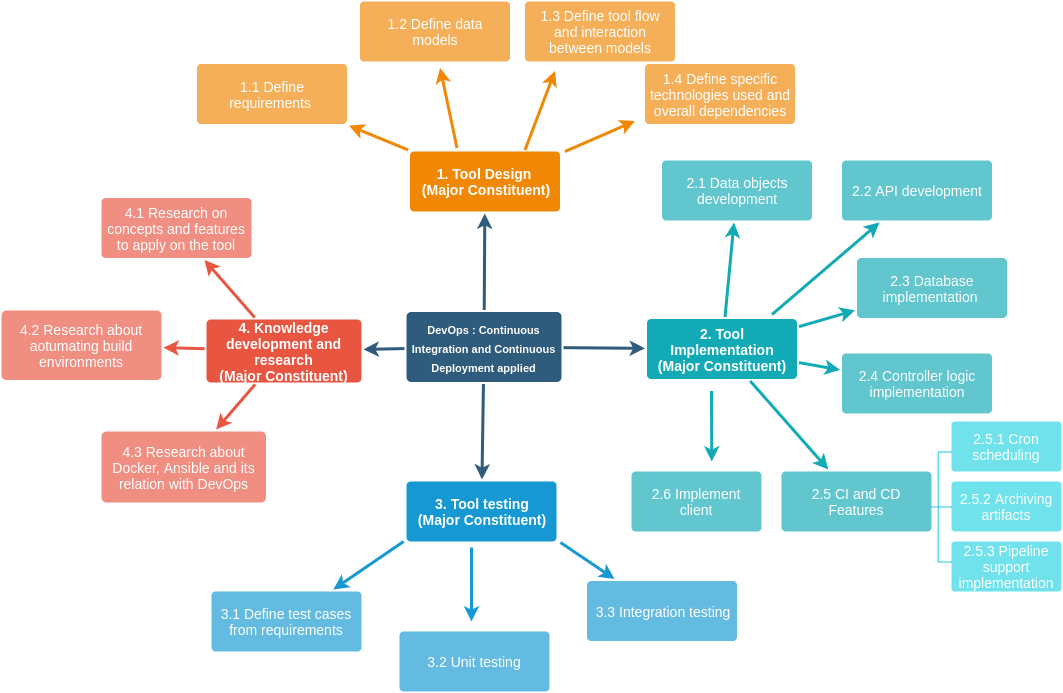
\includegraphics[scale=0.4]{wp_breakdown}
	\caption{Work Package breakdown, self-elaboration.}
\end{figure}
~\\
\begin{normalsize}
\setlength{\extrarowheight}{0pt}

\begin{table}[H]
\begin{tabularx}{\textwidth}{|X|c|}
	\hline
	\textbf{WP Name:} Define requirements& \textbf{WP ref: 1.1} \\ \hline
	\textbf{Major constituent:} Tool Design & - \\ \hline
	\multirow{2}{*}{\begin{tabular}[c]{@{}l@{}}\textbf{Short description:} Define specific requirements\\based on DevOps real world culture and concepts \end{tabular}} &  \textbf{Planned start date:} 16/Feb/2020\\ \cline{2-2} 
	&  \textbf{Planned end date:} 19/Feb/2020\\ \hline
\end{tabularx}
\caption{WP 1.1}
\end{table}
\begin{table}[H]
\begin{tabularx}{\textwidth}{|X|c|}
	\hline
	\textbf{WP Name:} Define data models& \textbf{WP ref: 1.2} \\ \hline
	\textbf{Major constituent:} Tool Design & - \\ \hline
	\multirow{2}{*}{\begin{tabular}[c]{@{}l@{}}\textbf{Short description:} Think about data models\\that will define the tool and its DB representation. \end{tabular}} &  \textbf{Planned start date:} 24/Feb/2020\\ \cline{2-2} 
	&  \textbf{Planned end date:} 26/Feb/2020\\ \hline
\end{tabularx}
\caption{WP 1.2}
\end{table}
\begin{table}[H]
\begin{tabularx}{\textwidth}{|X|c|}
	\hline
	\textbf{WP Name:} Define tool flow and interaction& \textbf{WP ref: 1.3} \\ \hline
	\textbf{Major constituent:} Tool Design & - \\ \hline
	\multirow{2}{*}{\begin{tabular}[c]{@{}l@{}}\textbf{Short description:} Define the application flow\\of the application and how the models will\\interact between them.  \end{tabular}} &  \textbf{Planned start date:} 26/Feb/2020\\ \cline{2-2} 
	& \multicolumn{1}{c|}{\begin{tabular}[c]{@{}c@{}}\\\textbf{Planned end date:} 27/Feb/2020\end{tabular}}\\ & \\ \hline
\end{tabularx}
\caption{WP 1.3}
\end{table}
\begin{table}[H]
\begin{tabularx}{\textwidth}{|X|c|}
	\hline
	\textbf{WP Name:} Define specific technologies and dependencies& \textbf{WP ref: 1.4} \\ \hline
	\textbf{Major constituent:} Tool Design & - \\ \hline
	\multirow{2}{*}{\begin{tabular}[c]{@{}l@{}}\textbf{Short description:} Define programming\\languages involved, general dependencies and\\technologies that will be used. \end{tabular}} &  \textbf{Planned start date:} 25/Feb/2020\\ \cline{2-2} 
	& \multicolumn{1}{c|}{\begin{tabular}[c]{@{}c@{}}\\\textbf{Planned end date:} 25/Feb/2020\end{tabular}} \\ 
	& \\ \hline
\end{tabularx}
\caption{WP 1.4}
\end{table}
\begin{table}[H]
\begin{tabularx}{\textwidth}{|X|c|}
	\hline
	\textbf{WP Name:} Data objects development& \textbf{WP ref: 2.1} \\ \hline
	\textbf{Major constituent:} Tool Implementation & - \\ \hline
	\multirow{2}{*}{\begin{tabular}[c]{@{}l@{}}\textbf{Short description:} Represent the data models\\in Python class and the database models as well. \end{tabular}} &  \textbf{Planned start date:} 02/Mar/2020\\ \cline{2-2} 
	&  \textbf{Planned end date:} 05/Mar/2020\\ \hline
\end{tabularx}
\caption{WP 2.1}
\end{table}
\begin{table}[H]
\begin{tabularx}{\textwidth}{|X|c|}
	\hline
	\textbf{WP Name:} API Developments& \textbf{WP ref: 2.2} \\ \hline
	\textbf{Major constituent:} Tool Implementation & - \\ \hline
	\multirow{2}{*}{\begin{tabular}[c]{@{}l@{}}\textbf{Short description:} Development of the API in\\order to make the models accessible from a client. \end{tabular}} &  \textbf{Planned start date:} 09/Mar/2020\\ \cline{2-2} 
	&  \textbf{Planned end date:} 24/Mar/2020\\ \hline
\end{tabularx}
\caption{WP 2.2}
\end{table}
\begin{table}[H]
\begin{tabularx}{\textwidth}{|X|c|}
	\hline
	\textbf{WP Name:} Database Implementation& \textbf{WP ref: 2.3} \\ \hline
	\textbf{Major constituent:} Tool Implementation & - \\ \hline
	\multirow{2}{*}{\begin{tabular}[c]{@{}l@{}}\textbf{Short description:} Implement the logic for\\accessing to the SQL database using Python. \end{tabular}} &  \textbf{Planned start date:} 03/Mar/2020\\ \cline{2-2} 
	&  \textbf{Planned end date:} 10/Mar/2020\\ \hline
\end{tabularx}
\caption{WP 2.3}
\end{table}
\begin{table}[H]
\begin{tabularx}{\textwidth}{|X|c|}
	\hline
	\textbf{WP Name:} Controller logic implementation& \textbf{WP ref: 2.4} \\ \hline
	\textbf{Major constituent:} Tool Implementation & - \\ \hline
	\multirow{3}{*}{\begin{tabular}[c]{@{}l@{}}\textbf{Short description:} Develop the logic for using\\the data models and giving capabilities for user\\interaction through the API.\end{tabular}} &  \textbf{Planned start date:} 08/Mar/2020\\ \cline{2-2} 
	& \multicolumn{1}{c|}{\begin{tabular}[c]{@{}c@{}}\\\textbf{Planned end date:} 29/Mar/2020\end{tabular}}\\ 
	&  \\ \hline
\end{tabularx}
\caption{WP 2.4}
\end{table}
\begin{table}[H]
\begin{tabularx}{\textwidth}{|X|c|}
	\hline
	\textbf{WP Name:} CI and CD Features& \textbf{WP ref: 2.5} \\ \hline
	\textbf{Major constituent:} Tool Design & - \\ \hline
	\multirow{2}{*}{\begin{tabular}[c]{@{}l@{}}\textbf{Short description:} Basing on the research done\\in parallel in WP 4.1 implement features. \end{tabular}} &  \textbf{Planned start date:} 30/Mar/2020\\ \cline{2-2} 
	&  \textbf{Planned end date:} 22/Apr/2020\\ \hline
	\multicolumn{2}{|l|}{\begin{tabular}[c]{@{}l@{}}\textbf{2.5.1 Cron scheduling}: Implementing capability to  schedule jobs periodically with \\ cron expressions\end{tabular}} \\ \hline
	\multicolumn{2}{|l|}{\begin{tabular}[c]{@{}l@{}}\textbf{2.5.2 Archiving artifacts}: Implementing capability to store binaries and outputs\\from build executions\end{tabular}} \\ \hline
	\multicolumn{2}{|l|}{\begin{tabular}[c]{@{}l@{}}\textbf{2.5.3 Pipeline support}: Implementing capability to define builds through YAML \\pipelines.\end{tabular}} \\ \hline
\end{tabularx}
\caption{WP 2.5}
\end{table}
\begin{table}[H]
\begin{tabularx}{\textwidth}{|X|c|}
	\hline
	\textbf{WP Name:} Implement Client& \textbf{WP ref: 2.6} \\ \hline
	\textbf{Major constituent:} Tool Implementation & - \\ \hline
	\multirow{2}{*}{\begin{tabular}[c]{@{}l@{}}\textbf{Short description:} Implement a client with GUI\\in order to interact with the API.\end{tabular}} &  \textbf{Planned start date:}24/Apr/2020\\ \cline{2-2} 
	&  \textbf{Planned end date:} 24/May/2020\\ \hline
\end{tabularx}
\caption{WP 2.6}
\end{table}
\begin{table}[H]
\begin{tabularx}{\textwidth}{|X|c|}
	\hline
	\textbf{WP Name:} Define test cases from requirements& \textbf{WP ref: 3.1} \\ \hline
	\textbf{Major constituent:} Tool Testing & - \\ \hline
	\multirow{2}{*}{\begin{tabular}[c]{@{}l@{}}\textbf{Short description:} Define test cases based on\\the requirements defined on WP 1.1 \end{tabular}} &  \textbf{Planned start date:} 21/May/2020\\ \cline{2-2} 
	&  \textbf{Planned end date:} 25/May/2020\\ \hline
\end{tabularx}
\caption{WP 3.1}
\end{table}
\begin{table}[H]
\begin{tabularx}{\textwidth}{|X|c|}
	\hline
	\textbf{WP Name:} Unit tests& \textbf{WP ref: 3.2} \\ \hline
	\textbf{Major constituent:} Tool Testing & - \\ \hline
	\multirow{2}{*}{\begin{tabular}[c]{@{}l@{}}\textbf{Short description:} Write unit tests for each\\module and function that is critical. \end{tabular}} &  \textbf{Planned start date:} 25/May/2020\\ \cline{2-2} 
	&  \textbf{Planned end date:} 27/May/2020\\ \hline
\end{tabularx}
\caption{WP 3.2}
\end{table}
\begin{table}[H]
\begin{tabularx}{\textwidth}{|X|c|}
	\hline
	\textbf{WP Name:} Integration Testing& \textbf{WP ref: 3.3} \\ \hline
	\textbf{Major constituent:} Tool Testing & - \\ \hline
	\multirow{2}{*}{\begin{tabular}[c]{@{}l@{}}\textbf{Short description:} Write integration tests\\checking overall tool functionality. \end{tabular}} &  \textbf{Planned start date:} 27/May/2020\\ \cline{2-2} 
	&  \textbf{Planned end date:} 29/May/2020\\ \hline
\end{tabularx}
\caption{WP 3.3}
\end{table}
\begin{table}[H]
\begin{tabularx}{\textwidth}{|X|c|}
	\hline
	\textbf{WP Name:} Research on concepts and features to apply on the tool& \textbf{WP ref: 4.1} \\ \hline
	\textbf{Major constituent:} Knowledge development and research & - \\ \hline
	\multirow{2}{*}{\begin{tabular}[c]{@{}l@{}}\textbf{Short description:} Read books and articles\\trending on the topic to conclude features that \\ might fit on the tool. \end{tabular}} &  \textbf{Planned start date:} 10/Mar/2020\\ \cline{2-2} 
	&  \multicolumn{1}{c|}{\begin{tabular}[c]{@{}c@{}}\\\textbf{Planned end date:} 04/Jun/2020\end{tabular}} \\
	& \\ \hline
\end{tabularx}
\caption{WP 4.1}
\end{table}
\begin{table}[H]
\begin{tabularx}{\textwidth}{|X|c|}
	\hline
	\textbf{WP Name:} Research about automating build environments & \textbf{WP ref: 4.2} \\ \hline
	\textbf{Major constituent:} Knowledge development and research & - \\ \hline
	\multirow{2}{*}{\begin{tabular}[c]{@{}l@{}}\textbf{Short description:} Strictly related to 4.3, get\\conclusions on this topic and write thoughts. \end{tabular}} &  \textbf{Planned start date:} 11/May/2020\\ \cline{2-2} 
	&  \multicolumn{1}{c|}{\begin{tabular}[c]{@{}c@{}}\\\textbf{Planned end date:}
			01/Jun/2020\end{tabular}}\\ 
	& \\\hline
\end{tabularx}
\caption{WP 4.2}
\end{table}
\begin{table}[!t]
\begin{tabularx}{\textwidth}{|X|c|}
	\hline
	\textbf{WP Name:} Research about Docker, Ansible and its relation with DevOps& \textbf{WP ref: 4.3} \\ \hline
	\textbf{Major constituent:} Knowledge development and research & - \\ \hline
	\multirow{2}{*}{\begin{tabular}[c]{@{}l@{}}\textbf{Short description:} Research and write ways in\\which these technologies can be used and applied. \end{tabular}} & \textbf{Planned start date:} 14/May/2020\\ \cline{2-2} 
	&  \textbf{Planned end date:} 02/Jun/2020\\ \hline
\end{tabularx}
\caption{WP 4.3}
\end{table}
\end{normalsize}
\clearpage
\subsection{Deviations from the initial plan and incidences}
~\\
Below you can see the current GANTT which slightly differs from the initial planning :

\begin{figure}[!h]
    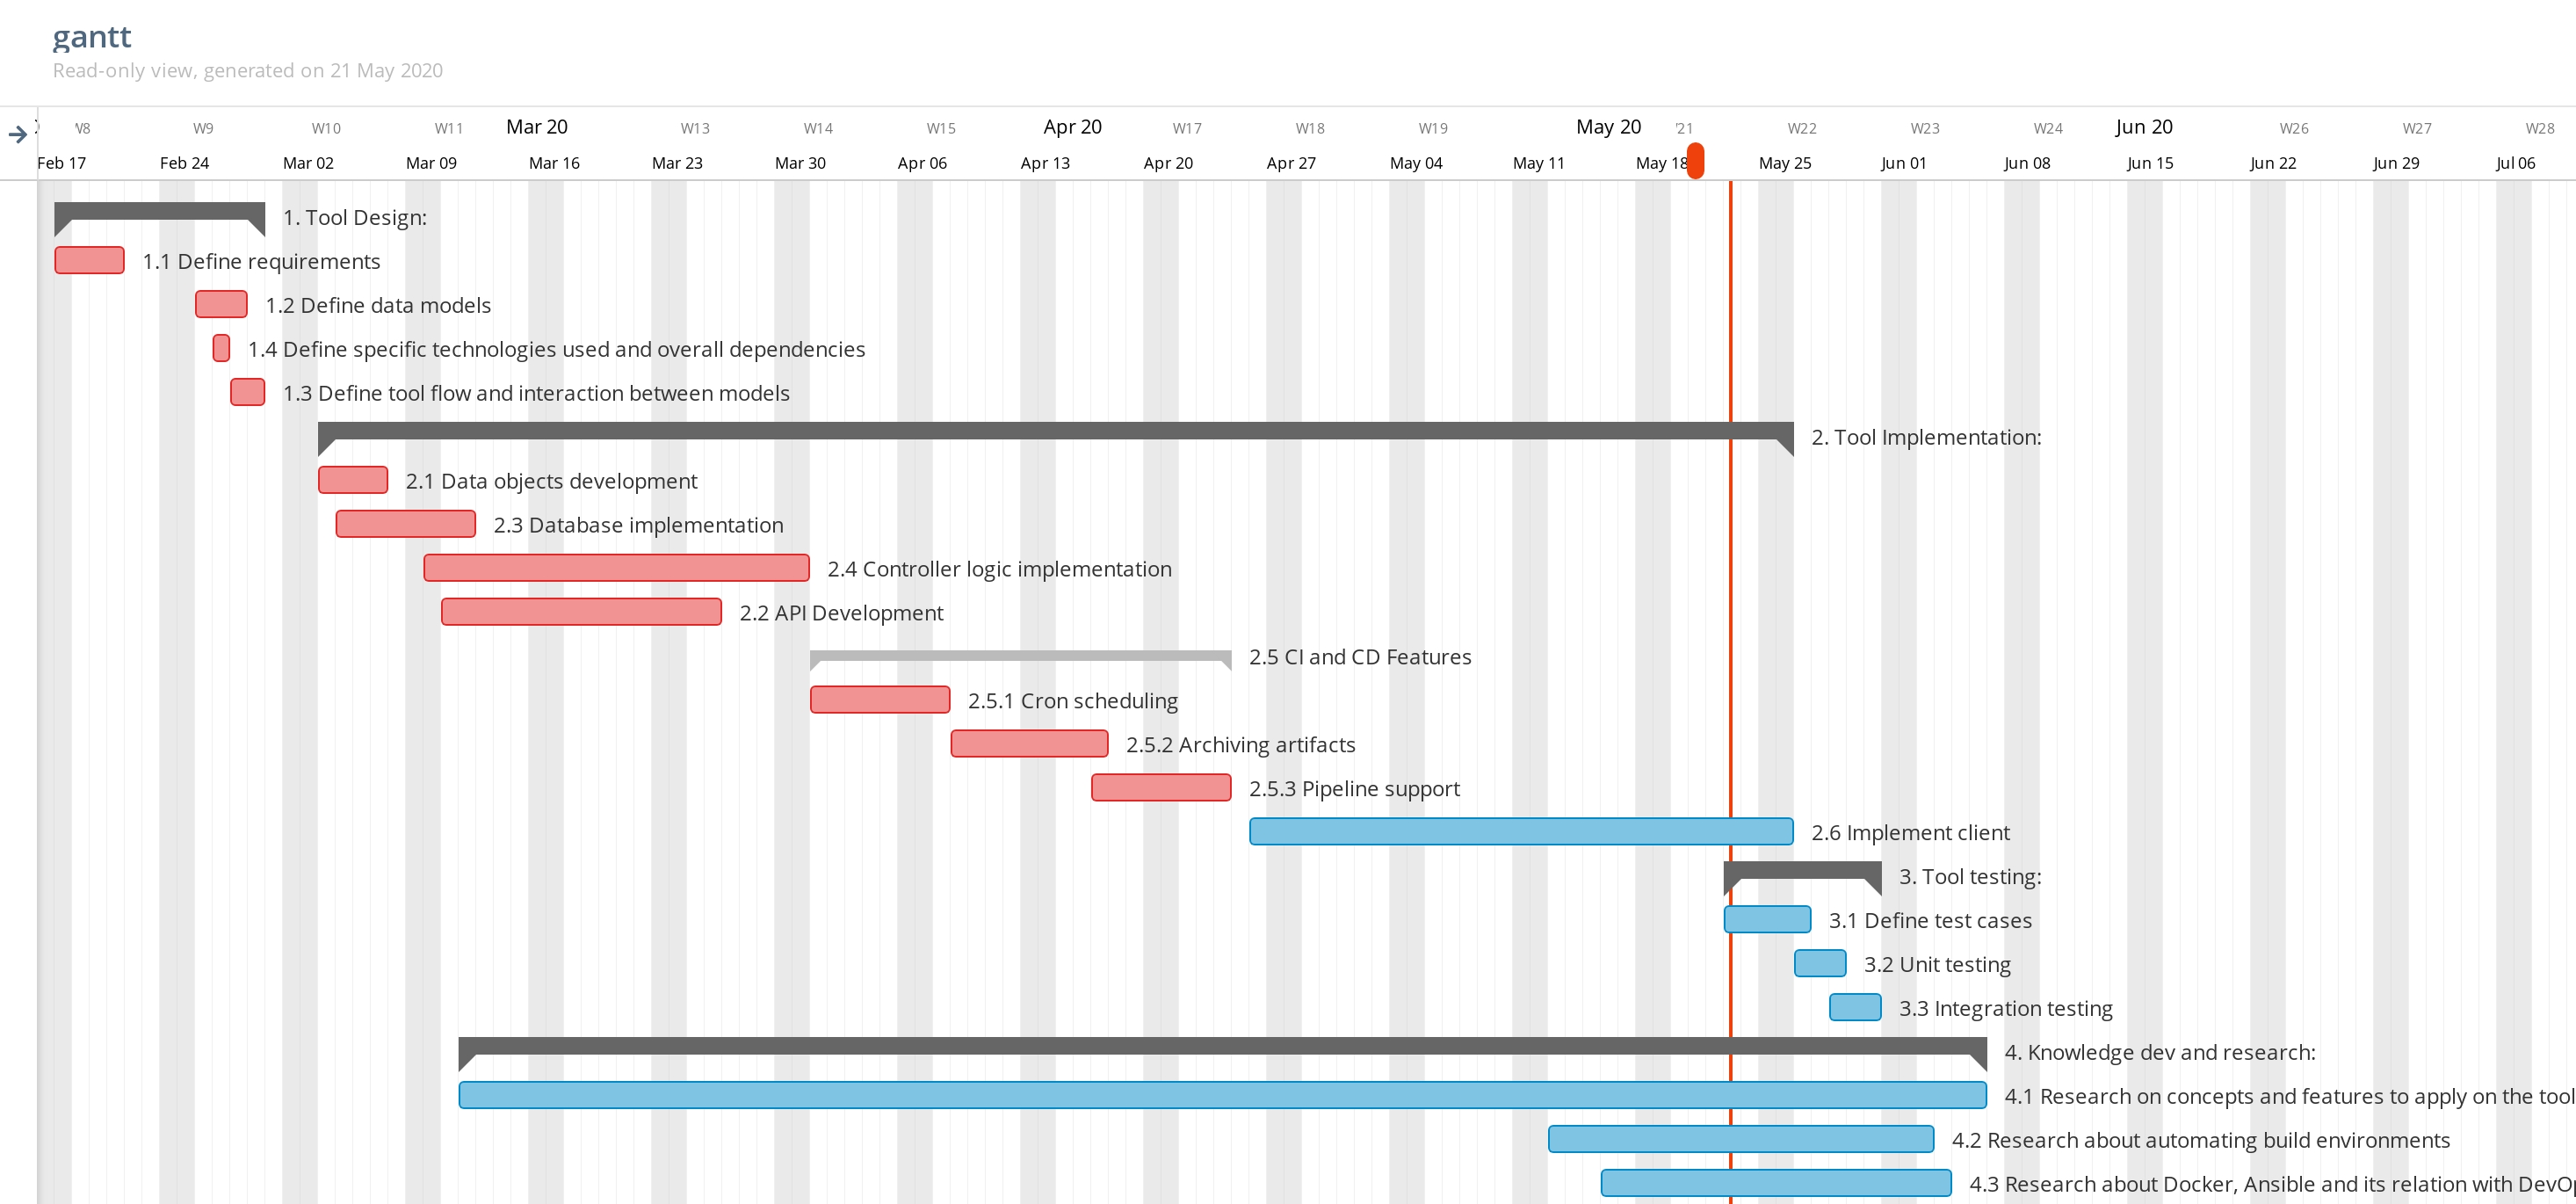
\includegraphics[scale=0.15]{gantt}
    \caption{GANTT diagram, self-elaboration.}
\end{figure}
~\\
The differences with the initial GANNT are the following : 

%\addcontentsline{lot}{table}{Differences with initial planning}
\begin{table}[H]
\begin{tabularx}{\textwidth}{|l|X|}
\hline
\textbf{WP} & \textbf{Reason} \\ \hline
\textbf{WP 2.6} & Client implementation duration has been extended by 4 days, developing front-end has been a challenge for me, as a Software Developer my skills are more related to back-end technologies, then I needed more time to complete the task. \\ \hline
\textbf{WP 3.4} & Automated testing task has been deleted, for the sake of simplicity while developing I decided to not automate the tests (with an external tool), but simply run them after every commit with a simple bash script that run the tests and then perform the commit if tests has passed. This could be considered in some way automated testing but still has a manual part. \\ \hline
\textbf{WP 4.1} &  In April the priority for this work package upgraded and I started dedicating more hours per week due to the reason that I was spending less time to researching on concepts and developing the knowledge on DevOps than developing the tool.\\ \hline
\end{tabularx}
\caption{Differences with initial planning}
\end{table}
\newpage
\section{State of the art of the technology used or applied in this thesis}

Before getting into DevOps state on nowadays SW industry I will talk about an even more important concept, which is the basis of everything related to DevOps, this is automation conceived as "the technology by which a process or procedure is performed with minimal human assistance", automation is the key for speeding and improving any process related to software, it allows all of the common tasks involved in the creation and deployment of software to be performed by developers, testers, and operations personnel, at the push of a button. Automation tools reduce labor, energy, and materials used to improve quality and accuracy of outcomes.
~\\
In the field of software we can distinguish between different types of automation :

\begin{itemize}
    \item Server Installation : Consists on setting up and configuring servers through automation.
    \item Infrastructure Automation : Basically, this consists in what is conceived as \gls{IaC}, an IT paradigm oriented to provision and deploy infrastructure with code, just as the rest of your software. Tools such as Ansible have this purpose as a goal.
    \item Test and Build Automation : This is the field the thesis mainly focuses on, test and build automation tools make possible to keep developing without having our work laptop frozen due to RAM or CPU run out when compiling a big project, this kind of tools make possible to connect slave nodes in which the builds will take place so the developers don't have to run the build processes locally on their computers. Also is a good practice for having centralized all the builds of a project as well as its resulting binary artifacts, and opens the door to DevOps world. There are also different types of build and tests automation which will be seen along the thesis : 
    \begin{itemize}
        \item On-demand automation : In this case the build is triggered by the user.
        \item Scheduled automation : This kind of automation gives rise to the known nightly builds, the builds are scheduled often through Cron Expressions, this makes possible running builds when no-one is working on the project in order to build all the changes commited by the developers along the day.
        \item Triggered automation : This is strictly related to \gls{VCS} such as Git or Svn, this kind of automation trigger builds depending on the workflow followed, for example if the project follows a feature branching git model, builds or tests can be triggered when pull requests to master are merged, or even with every commit performed by the developers.
    \end{itemize}
\end{itemize}
\newpage
~\\
Let's introduce the DevOps concept itself with an example, imagine your first days as a developer in a company on a field you have already experience in, you get your laptop with the propper development environment setup. After you write some new code you perform a commit and these changes are queued to be built and tested against a server which contains the build environment setup, if tests passes now you have a certain degree of confidence that the new code is correct and you can decide (depending on the complexity and other factors) whether to open a Pull Request, which will be submitted to a code review, in order to bring these changes to production environment. 
\vspace{5px}
~\\
The duration of all this processes can vary depending on the project size, it is so common that can be done more than 5 times a day per developer (see in the following table typical deployment frequencies) so the steps followed must be efficient and well structured. The wrap up of all this processes is conceived as Pipeline or DevOps pipeline, a pipeline consists of a set of tools, flows, and automated processes, enabling teams to to build and deploy software efficiently, and includes Continuous Integration and Continuous Deployment.

\begin{table}[H]
\centering
\begin{tabular}{|l|l|}
\hline
\textbf{Company} & \textbf{Deployment Frequency} \\ \hline
Amazon           & 23,000 per day                \\ \hline
Google           & 5,500 per day                 \\ \hline
Netflix          & 500 per day                   \\ \hline
Facebook         & 1 per day                     \\ \hline
Twitter          & 3 per week                    \\ \hline
Typical Company  & 1 every 9 months              \\ \hline
\end{tabular}
\caption{Software Deployment Frequency on diverse companies, source : The Phoenix Project}
\end{table}
\noindent
DevOps is not just another software development methodology, is a way of thinking and operating that enable teams to deploy software in efficient and lasting ways, it is part of the culture that shapes how and why we work, a philosophy of close collaboration between traditionally distinct disciplines, the Development team and the Operations team.
\vspace{5px}
~\\
A merge of Development and Operations teams conceiving the DevOps team, becomes a requirement on most of nowadays projects and companies on the software field, in order to avoid deployment failures produced by the increase of complexity:
\begin{aquote}{Collaborative DevOps with Rational and Tivoli, 2011 IBM}
A key factor that has led to the high level of deployment failures we see today is a corresponding increase in software and infrastructure complexity over time ... Overcoming all this complexity requires a tremendous amount of coordination and communication.
\end{aquote}
\newpage
Moving into more specific DevOps related concepts, Pipelines, Continuous Integration and Continuous Deployment will be defined more in detail.

The following image describes the steps of a general DevOps loop cycle or pipeline: 
\begin{figure}[H]
    \centering
    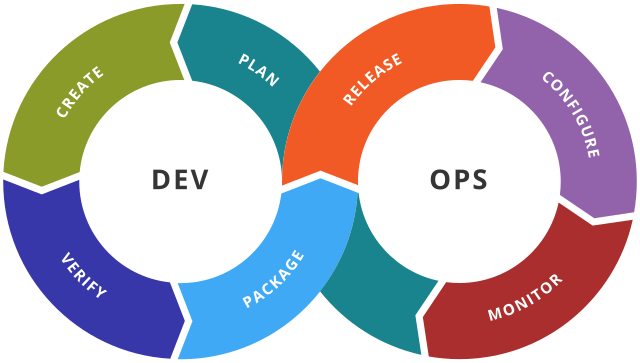
\includegraphics[scale=0.2]{devops_loop}
    \caption{DevOps loop, author:
    \href{https://commons.wikimedia.org/wiki/File:Devops-toolchain.svg}{Kharnagy}}
\end{figure}
All the steps in the image above are simple and easy to understand, but are also complex when it refers to proceed with a project, each of them implies the usage of certain tools, going step by step some will be mentioned :


\begin{table}[H]
\centering
\begin{tabular}{|l|c|l|l|}
\cline{1-1} \cline{3-4}
\multirow{8}{*}{\textbf{\begin{tabular}[c]{@{}l@{}}D\\ E\\ V\\ O\\ P\\ S\end{tabular}}} & \multicolumn{1}{l|}{}        & \textbf{Step} & \textbf{Tool}               \\ \cline{3-4} 
                                                                                        & \multicolumn{1}{l|}{}        & Plan          & Jira, VersionOne            \\ \cline{2-4} 
                                                                                        & \multirow{2}{*}{\textbf{CI}} & Create        & PyCharm, Visual Studio Code \\ \cline{3-4} 
                                                                                        &                              & Verify        & JUnit, Selenium             \\ \cline{2-4} 
                                                                                        & \multirow{3}{*}{\textbf{CD}} & Package       & Artifactory, Docker Hub     \\ \cline{3-4} 
                                                                                        &                              & Release       & Docker, AWS                 \\ \cline{3-4} 
                                                                                        &                              & Configure     & Ansible, Chef               \\ \cline{2-4} 
                                                                                        & \multicolumn{1}{l|}{}        & Monitor       & Datadog                     \\ \cline{1-1} \cline{3-4} 
\end{tabular}
\caption{DevOps toolchain}
\end{table}
\noindent
Continuous Integration is conceived as a software development practice where project members integrate their work often, where the frequency can go up to multiple integrations per day. With CI, code changes are integrated into a central repository several times a day. As a result, merging the different code changes from each developer becomes easier and less time-consuming. Bugs will also be encountered early and this will make it easier to resolve them. Referring to above pipeline model Continuous Integration would include the whole Create step, which can be splitted into code and build and also would include the Verify step. 
\vspace{5px}
~\\
Continuous Deployment is the process of deploying changes into production environment by minimizing the risk of failure, having passed a set of tests. You increase the frequency of releasing new features. Consequently, it enhances the customer feedback loop, hence creating the opportunity for better customer involvement. Regarding the pipeline model defined above, it would include the Package, Release and Configure steps.

\newpage
\noindent
Focusing on the tool that has been developed along this thesis, it is mainly written in Python, which I had to learn in order to proceed, chosen due to its huge amount of frameworks that eases the development and its learning curve. The minimum Python version required for running the tool is Python v3.6 as specified in the requirements. 
~\\

Web frameworks was the main focus for developing the tool, as a back-end REST API was one of the requirements, a web framework is a code library that makes web development faster and simpler by providing common patterns for building reliable and maintainable web applications. A REST API simply consists on building a service by specifying a set of operations on top of HTTP Protocol by using its methods (GET, POST, PUT and DELETE). The web framework chosen in order to proceed with the tool development is Flask, the reasons will be detailed in Methodology/Project Development section.
~\\

Also database related concepts had to be studied in order to carry out the tool development, as the tool itself requires the capability to store jobs and builds, I decided to focus the research only on relational type databases, avoiding NoSQL databases such as MongoDB for sack of simplicity at the moment of linking and creating relations between tables, and also because the database structure was clear and well defined from the beginning of the project. Finally, sqlite was the \gls{RDBMS} chosen over other SQL database engines since sqlite is not a client-server database, it is embedded into the end application.
~\\

In order to schedule jobs periodically inside the tool, which is a requirement, I decided to use cron expressions, as I am familiar with Unix systems, so I had to find a way to schedule code execution on Python using cron expressions. Eventually, one the libraries which allows this kind of code scheduling on Python is called Advanced Python Scheduler. 
~\\ 

Regarding the front-end, the requirement was to ease the usage of the tool, then something simple and lightweight was necessary. A single page app was created with Flask, the content of which changes dinamically, by performing queries to the back-end REST API, and by using a web template engine called Jinja and JQuery.


\newpage
\section{Methodology/Project Development}
\subsection{Design}
Along this section the methodologies and the practices used in the tool development and the project research will be described in detail.
~\\

The first weeks of the project it was under a design phase in which I created the whole specification for the tool development, the requirements exposed at the beginning of the thesis, and also the toolchain which would be used. Basically I wanted to create a lightweight, portable, easy to deploy and OS independent tool with CI and CD features. 
~\\

The tool is an automation server that allows the user to schedule builds on-demand and get the build outputs, consisting on a back-end designed under an MVC pattern an a simple front-end in order to speed up the usage of the tool.
~\\

The CI features the tool has are the following :

\begin{itemize}
    \item \textbf{Job Scheduling} : The tool is capable of scheduling periodically builds using cron expressions.
    \item \textbf{Pipeline support} : The commands that will be run in a build can be contained in a YAML file ordered by stages in order to have a clear order and sense of the what will be happening in the build.
\end{itemize}

These features are grouped into Continuous Integration because they ease the process of testing a project and increases the build frequency in order to find bugs in less time, apart from automating the whole process.
~\\

Regarding the CD features of the tool :

\begin{itemize}
    \item \textbf{Artifacts archiving} : The tool is capable of storing binaries or any kind of output that a build produces, selectable by the user, for example after the build of a C project you can store all *.o and *.ar files.
\end{itemize}

This Continuous Deployment is a must in any DevOps tool, as it closes the loop, after the build is automated and the outputs are stored, we can deploy or deliver this output to the client, flash it to some hardware, monitor parameters. Hence, joining the CI and the CD features the DevOps loop is closed efficiently with the usage of the tool.


\newpage
\subsection{Implementation, dependencies and toolchain}

In this section we will see in detail the tool by reviewing the use cases for each dependencies and also an architecture overview that will be related with the previous dependencies explanation in order to fully understand the tool purpose and usage.
~\\

The tool has been developed with git as VCS in order to keep a clean change history, apart from the local index (where I stored all the changes), a github repostiory has been used as platform in some cases to push the changes (when I needed to share the work to another computer or work station). There is one repository for the frontend : https://github.com/HectorPascual/ci-cd-client and another one for the backend : https://github.com/HectorPascual/ci-cd-tool.
~\\

The tool has been implemented in Python using libraries and frameworks that have eased the process of development, in the following diagram you will see the toolchain used :
~\\

\begin{figure}[H]
    \centering
    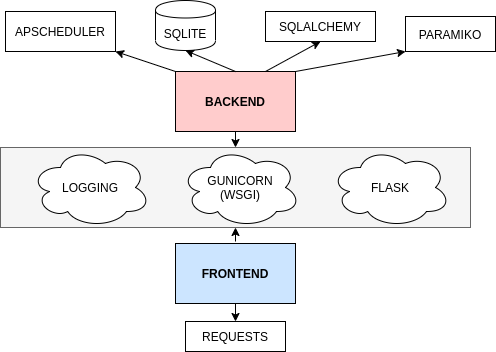
\includegraphics[scale=0.6]{tfg_toolchain}
    \caption{Toolchain used, self-elaboration}
\end{figure}

The dependencies in the diagram will be briefly explained and justified for the use case :

\subsubsection{APSCHEDULER}

Is a Python library that lets you schedule code pieces defined as jobs, in concrete I am using an instance of the object BackgroundScheduler in order to run pieces of code in background while running the application.

The following piece of code schedules a build, the piece of code scheduled is contained in create\_build function, parsed as first argument, then we use kwargs in order to pass the arguments regarding the create\_build function, with trigger parameter we specify the type of trigger, in the case of our tool we want to use cron expresions, then we specify the cron parameters (minute, hour, day, month and day of week) finally an id that will identify the job and then we start the scheduler:

\begin{lstlisting}[language=Python]
scheduler.add_job(func=create_build, kwargs=kwargs, trigger="cron", 
                  minute=minute, hour=hour, day=day_month, month=month, 
                  day_of_week=day_week, id=cron_key)
scheduler.start()
\end{lstlisting}
\subsubsection{SQLITE}

Is a very lightweight and easy to include type of database and I decided to use it on the tool, the database is automatically created if there's none on the base directory of the tool.

\subsubsection{SQLALCHEMY}

SQLAlchemy is a framework that eases Python management of \gls{SQL} databases, on our main app file we create a database object using SQLAlchemy constructor, this will allow us to perform operations and define schemas for the database.

\begin{lstlisting}[language=Python]
from flask_sqlalchemy import SQLAlchemy
# ...
# app object initialization
# ...

# specify db path
app.config['SQLALCHEMY_DATABASE_URI'] = 'sqlite:///' + os.path.join(
    os.path.dirname(os.path.dirname(__file__)), 'app.db') 
# db object initialization
db = SQLAlchemy(app) 
\end{lstlisting}

We use the db object mainly for defining the schemas (models) for the data types that will be stored in the database, for instance, a job is represented the following way in the database :

\begin{lstlisting}[language=Python]
import datetime
from src.app import db


class Job(db.Model):
    id = db.Column(db.Integer, primary_key=True)
    title = db.Column(db.Text)
    description = db.Column(db.Text)
    created_date = db.Column(db.DateTime, default=datetime.datetime.utcnow)

    builds = db.relationship('Build', backref='job', lazy = False)
    # ...
\end{lstlisting}

Basically the models consists of a primary key, which is the id, the properties and then we are taking profit of SQL relationships between tables, a Job can contain multiple builds.

Note that we are not taking profit of lazy loading capability of SQLAlchemy, we are using \textit{Eager} loading which specifies that you always want to retrieve the relationship, not only when the object is being accessed.

\subsubsection{PARAMIKO}

Paramiko is the \gls{SSH} Python library by reference, it contains an SSH client and server implementation and allows you to perform all SSH operations through Python code.

The use case for the tool is basically creating SSH connections to nodes where the builds can be executed.

Not only I am taking profit of the SSH connection for executing commands but also sharing files between the slave node and the master (which is the one that hosts the tool) in order to retrieve binary files and results of certain builds, by using SFTP protocol over SSH.

In the tool architecture, which will be seen in the next subsection, there's the concept of Runner, which is an object that allows a node to run commands and perform SSH operations. Its definition using Paramiko is as follows : 


\begin{lstlisting}[language=Python]
class RunnerSSH():
    def __init__(self, node):
        self.node = node
        self.ssh_client = paramiko.SSHClient()
        self.ftp_client = None

    def connect(self):
        try:
            self.ssh_client.set_missing_host_key_policy(paramiko.AutoAddPolicy)
            self.ssh_client.connect(self.node.ip_addr, self.node.port, self.node.user, self.node.password)
            logging.info("[SSH] Connection established successfully")
        except Exception as e:
            logging.warning(f'[SSH] There was an error while establishing connection {e}')

    def run_commands(self, commands):
        output = ""
        cmd_list = commands.split(';')
        status = "passed"
        for cmd in cmd_list:
            logging.info(f"Executing shell command : {cmd}")
            _ , stdout , stderr = self.ssh_client.exec_command(f"cd {self.node.workspace};{cmd}")
            output += stdout.read().decode("utf-8") +  stderr.read().decode("utf-8") + '\n'
            if stderr.channel.recv_exit_status() != 0:
                status = "failed"
        return output, status

    def get_files(self, artifacts, local_path, workspace):
        # Create local path if doesn't exist
        Path(local_path).mkdir(parents=True, exist_ok=True)

        # Init sftp session if not existing yet
        if not self.ftp_client:
            self.ftp_client = self.ssh_client.open_sftp()
        # Logic for obtaining files ...
        # ...

\end{lstlisting}

The SSH Runner class allows connecting to a node, running commands on the node as well as setting a failed build status in case any command returns an error code, and getting files on a certain workspace using wildcards and specifying the file extension.

\subsubsection{LOGGING}

Python's logging module is included in the standard library, and is such a powerful tool for emitting different kind of messages through configuring different log handlers and a way of routing log messages to these handlers on scripts and applications.
~\\

The use case for the tool is basically having different levels of logging, so the output of the app is more traceable and readable. Logging module also allows to configure the format of the messages and select which is the default level of the mentioned below. The app will ignore any message with less level than the selected one.

\begin{table}[H]
\centering
\begin{tabular}{|l|l|}
\hline
\textbf{Level} & \textbf{Numeric value} \\ \hline
ERROR           & 40                \\ \hline
WARNING           & 30               \\ \hline
INFO          & 20               \\ \hline
DEBUG         & 10                     \\ \hline
\end{tabular}
\caption{Log levels used in the tool, source : Python docs}
\end{table}

\subsubsection{GUNICORN}

The tool can be directly launched with Flask, but according to Flask documentation : "This launches simple builtin server, which is good enough for testing but probably not what you want to use in production". Even though the builtin server is good for demos and testing, I decided to go deeper into this topic and use a real \gls{WSGI}. 
~\\

As I am a UNIX environments user I chose Gunicorn for my productive environment, but any other WSGI such as mod\_wsgi from apache or uWSGI can be used. 
~\\

Gunicorn is an HTTP Server that meets WSGI specification an allows serving Flask applications with multiple workers in order to increase the performance of our application.
~\\

In the tool deployment I am using the most basic workers type, a synchronous worker, that handles a single request at a time. But this does not mean poor requests handling per second, as it is bound to the CPU, with good hardware it can handle even hundreds or thousands requests per second with between 4 and 12 workers.
~\\

For instance, in order to run the backend we use the following bash cmd :  

\begin{lstlisting}
$ gunicorn -b localhost:5000  -w 4 src.app:app 
\end{lstlisting}

Where -b flag is used to bind a server socket in this case we are deploying to localhost in port 5000.

\subsubsection{FLASK}

Flask is the basis for both the front-end and the back-end, it allows to prototype a REST API well defined relatively fast and the usage of blueprints eases the creation of a modular application.

Basically the whole tool spins around the app object, defined in the main app module :

\begin{lstlisting}[language=Python]
from flask import Flask
from src.api import api_blueprint

app.register_blueprint(api_blueprint)
app = Flask(__name__)
\end{lstlisting}

The blueprint allow to define routes in other modules. For instance, the module which contains all the routes in the back-end looks as follows : 

\begin{lstlisting}[language=Python]
from flask import Blueprint, Response, request
import logging

logger = logging.getLogger('root')

api_blueprint = Blueprint('api', __name__)

@api_blueprint.route('/jobs', methods=('GET', 'POST'))
def jobs():
# ...

@api_blueprint.route('/jobs/<int:job_id>', methods=('GET', 'DELETE'))
def job(job_id):
# ...

@api_blueprint.route('/jobs/<int:job_id>/builds', methods=('GET', 'POST'))
def builds(job_id):
# ...

@api_blueprint.route('/nodes', methods=('GET', 'POST'))
def nodes():
# ...
\end{lstlisting}

As it is shown above, the blueprint allows to define routes in a different module, the API methods will be seen in detail in the following subsection.

\subsubsection{REQUESTS}

Requests is an elegant and simple HTTP Python library, the use case for the tool is widely found on the front-end code, in order to perform REST API operations agains't the backend.

For instance, in the next piece of code from the front-end code, the handler for a build route can be seen, basically it performs an operation agains't the backend and gets the required data, finally renders the template with the data fulfilled.

\begin{lstlisting}[language=Python]
@app.route('/jobs/<int:job_id>/builds/<int:build_id>')
def build(job_id, build_id):
    build = requests.get(f'http://localhost:5000/jobs/{job_id}/builds/{build_id}').json()
    node_id = build['node_id']
    node = requests.get(f'http://localhost:5000/nodes/{node_id}').json()
    return render_template("index.html", node=node, build=build)
\end{lstlisting}

\subsection{Implementation, project architecture}

Basically the tool consists on a front-end and a back-end which runs independently with different sockets bound, this decision was taken for being able to bring up the client locally in any machine and connect it to a centralised back-end that can be hosted on a dedicated server or virtual machine.

The back-end consists on a REST API capable of automating builds with the following structure defined :

\begin{figure}[H]
    \centering
    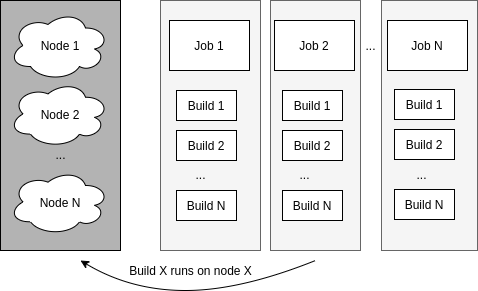
\includegraphics[scale=0.6]{basicarch}
    \caption{Simple back-end jobs structure, self-elaboration}
\end{figure}

Above diagram leads to the definition of the concepts mentioned :

\subsubsection{Job}

A job in the tool is conceived as a folder or way to group builds of a same project with a similar purpose. For instance, we could have a job which contains nightly builds and run tests on a project. I have given jobs the only purpose to serve as containers of different kind of builds, so a same job could store compiling builds and test builds.


\subsubsection{Build}
A build stores the configuration and description of a set of commands that might accomplish a purpose on a project (i.e : run tests, build project ...), in the tool there are two kinds of builds, the regular ones and the cron builds, this last type allows to schedule the build to be repeated based in a Cron Expression. Every build has a status which can be passed or failed depending on the return code returned by the commands run.
~\\

As explained, builds are based on a set of commands, but there are two ways in the tool to specify this commands, the first one consists on passing all the commands in the following format :
\vspace{0.2cm}
~\\
\textit{command1;command2;...;commandN}
\vspace{0.2cm}
~\\
The second way of passing commands consists of a Pipeline, a YAML file the structure of which is defined by stages, a stage is a group of commands which can have a name that gives a generic reference of what are these commands doing, so the overall set of commands is much easier to read and understand. A pipeline example looks as follows :

\begin{lstlisting}[language=yaml]
---
- stage:
    name: Checkout
    commands :
        - git clone https://github.com/HectorPascual/ci_cd_tool.git
        - echo 'hello'

- stage:
    name: Build
    commands:
        - pwd
        - ls
        - time
        - echo bye

- archive: 'ci-cd-tool/*.py'
- archive: '*.key'
---
\end{lstlisting}

\subsubsection{Node}

A node is where the builds takes place, basically a machine, the tool is capable of running builds on two types of nodes, the localhost node and SSH nodes. Localhost node is basically the machine where the tool is hosted, and the SSH nodes is any machine that has SSH capabilities (internet connection and an SSH protocol implementation), for testing purposes with the tool I used virtual machines.
~\\
~\\
The back-end software architecture is based on an MVC pattern, see the backend structure :

\begin{lstlisting}[style=ascii-tree]
├── app.db
├── artifacts/
│   └── job_2/
│   │   ├── build_39/
│   │   └── build_40/      
├── Pipfile
├── Pipfile.lock
├── README.md
├── src/
│   ├── app.py
│   ├── runner.py
│   ├── api/
│   │   ├── api_routes.py
│   │   └──__init__.py
│   ├── controller/
│   │   ├── build_controller.py
│   │   ├── cron_controller.py
│   │   ├── __init__.py
│   │   ├── job_controller.py
│   │   └── node_controller.py
│   ├── __init__.py
│   └── schemas/
│       ├── build.py
│       ├── cron_build.py
│       ├── __init__.py
│       ├── job.py
│       └── node.py
└── tests/
    └── test.yaml
\end{lstlisting}

First of all, we find the sqlite database where the data of the tool is stored, then an artifacts folder where all the artifacts archived from a build are stored with the job structure in order to clarify the origin of each artifact, then we find the Pipfile and the Pipfile.lock, which will be described in detail :

\subsubsection{Pipenv}

In order to run the tool in a fast an easy way on any environment and not worrying about dependency installation, we are using Pipenv, which automatically creates and manages a virtual environment,by removing or adding packages from the Pipfile as you install uninstall packages inside the virtual environment. It also generates a Pipfile.lock, which is used to produce deterministic builds by storing hash codes and relevant data about the dependencies versions.

Installing all the dependencies of the tool with pipenv is as fast as typing the following command in the project directory :

\begin{lstlisting}
$ pipenv install
\end{lstlisting}

For instance, in order to enter the virtual environment and bring up the back-end the procedure would be the following :

\begin{lstlisting}
$ pipenv shell
$ gunicorn -b localhost:5000  -w 4 src.app:app
\end{lstlisting}

~\\
~\\
\noindent
Following the tree, we get to the src/ folder where all the source code is contained, where the app.py which is the main file where the db object and the app object are initialized and the runner.py already referenced before where all regarding node SSH connections and node localhost are described. Also 3 directories are present, api/ which is where all the routes are defined using Flask blueprints (would fit the View part on an MVC pattern), the controller/ and finally the schemas (which would fit the model part on an MVC pattern).

Controller files contains the logic for accessing the database and handling the data based on the models defined in the schemas. For instance, build\_controller.py contains the following functions :

\begin{lstlisting}[language=Python]
def get_builds(job_id, build_id=None):
    # ...

def create_build(job_id, commands, node_id, description, artifacts=''):
    # ...

def delete_build(job_id, build_id):
    # ...

def parse_yaml(cmd_file): # Pipeline parser (utility function)
    # ... 
\end{lstlisting}

Schemas files contains the database columns definition for every type of structure, also functions for parsing the object to string and to a Python dictionary, for instance Job schema looks as follows :

\begin{lstlisting}[language=Python]
import datetime
from src.app import db

class Job(db.Model):
    id = db.Column(db.Integer, primary_key=True)
    title = db.Column(db.Text)
    description = db.Column(db.Text)
    created_date = db.Column(db.DateTime, default=datetime.datetime.utcnow)

    builds = db.relationship('Build', backref='job', lazy = False)

    def to_dict(self):
        return {
            'id' : self.id,
            'title' : self.title,
            'description': self.description,
            'created_date': self.created_date.strftime("%m/%d/%Y, %H:%M:%S")
        }

    def __repr__(self):
        return f"<id {self.id}, description : {self.description}>"
\end{lstlisting}

The front-end consists on a single page flask application, which renders HTML code dynamically using Jinja2 and request python lib for performing HTTP operations agains't the back-end.

\begin{lstlisting}[style=ascii-tree]
├── app.py
├── Pipfile
├── Pipfile.lock
├── static
│   ├── css
│   │   └── index.css
│   └── js
│       └── index.js
└── templates
    └── index.html
\end{lstlisting}

Front-end repository structure is quite simple, we have (as before) the app.py where this time we also have the routes (no use of blueprints) for sack of simplicity, the Pipenv related files for the virtual environment and the dependencies, and then a static folder, where all the static files that will be served by the application are stored (for instance, the css code but also images or icons). The templates folder contains the main HTML file which not only contains HTML code but also is plenty of Jinja2 syntax in order to render the template.
~\\

In order to understand how the front-end renders the data an example regarding nodes is going to be exposed. First, the route is defined in the app.py module :

\begin{lstlisting}[language=Python]
@app.route('/nodes')
def nodes():
    nodes = requests.get('http://localhost:5000/nodes').json()
    return render_template("index.html", nodes=nodes)
\end{lstlisting}

As it can be seen, the render\_template function is used to server a static page with dynamic content (keyword arguments) by providing the name of the template and the variables you want to pass to the template engine as keyword arguments.
~\\

Then in the template we can handle the nodes variable using Jinja syntax, for instance :

\begin{lstlisting}[language=HTML]

      
      <a id="node_link{{ node.id }}">
        <div class="item">
          {{ node.id }} {{ node.workspace }} {{ node.ip_addr }} {{ node.user }}
        </div>
      </a>
    

\end{lstlisting}

The flow of an action would be, a user clicks on the front-end on a button, then a GET method is performed agains't /nodes route on the front-end, inside the route handler the data is queried to the back-end and the template is rendered by passing the nodes variable, once in the template with the usage of Jinja we display a list of nodes. Graphically, the flow simplified looks as follows :

\begin{figure}[H]
    \centering
    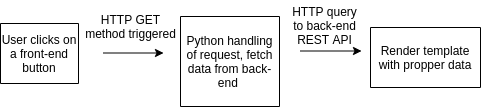
\includegraphics[scale=0.6]{frontendflow}
    \caption{Action flow example, self-elaboration}
\end{figure}

\newpage
\subsection{Testing}

Testing is a fundamental part on any application development, so basic that many companies nowadays are switching their development strategies to the usage of \gls{TDD} (Test Driven Development) which consists on creating tests from a developer’s perspective, this is the case of Thoughtworks, they got many articles on their website sharing thoughts about practices on TDD \footnote{Thoughtworks article about TDD  \url{https://www.thoughtworks.com/insights/blog/test-driven-development-best-thing-has-happened-software-design}.}. This  methodology  focuses  specifically  on  unit  tests based on the requirements,  then  the  code  is  written  by  the developer to pass those test cases. 
~\\
~\\
The development of this tool can't be considered fully that it has been under a TDD methodology, but I have shared some of the principles of it, such as think test cases from the requirements at the design part and test each case passes successfully once the development finished, the difference with TDD though, is that the even the cases were planned at design part, they were defined after the development part was over.
~\\
~\\
Testing can be split into 2 big groups, functional testing, which ignores internal parts and focuses only on the output, and non-functional testing which focuses on testing non-functional requirements such as Load Testing, Stress Testing, Security, Volume. Between these 2, groups we can distinguish a big variety of testing procedures. 
~\\
~\\
The tests performed on the tool are basically integration and unit tests (both types are functional tests). The difference between those two types of tests is simple and fundamental, unit tests are designed for testing small and specific parts of the tool, while integration testing is done to demonstrate that different pieces of the tool work together. 

~\\
~\\
The main focus for the tests was the back-end REST API, tested using Postman, which is an API client designed for testing and speed up the building of API's. With Postman you can easily store your HTTP requests ordered by collections, and compare the responses with the responses you expect, as well as checking correct behavior and testing some specific behaviors of your application under wrong requests or rare uncommon cases. In the following images, it can be seen an HTTP GET example and an HTTP POST example performed with Postman.

\begin{figure}[H]
    \centering
    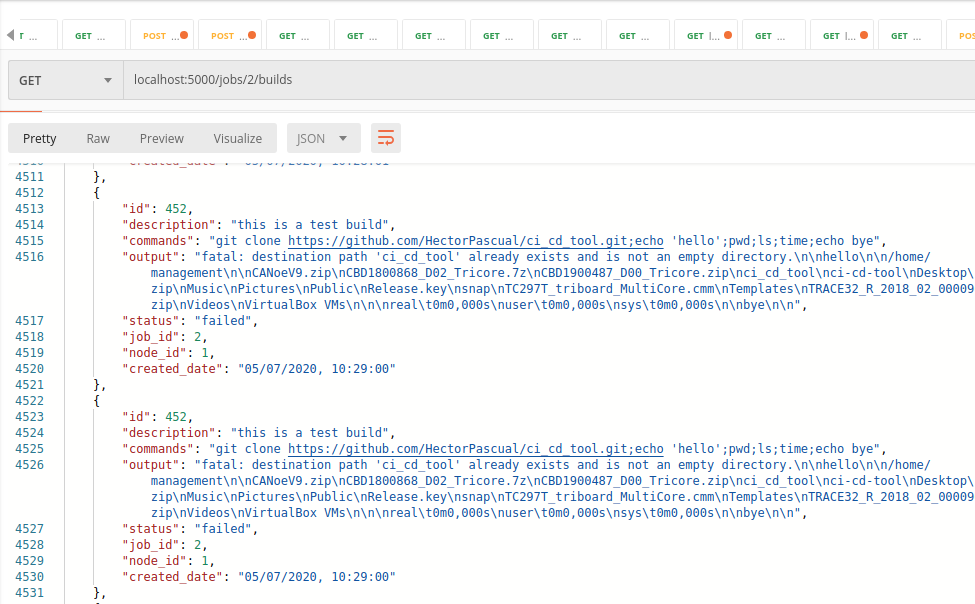
\includegraphics[scale=0.4]{postman_example1}
    \caption{HTTP GET example performed with Postman, self-elaboration}
\end{figure}

\begin{figure}[H]
    \centering
    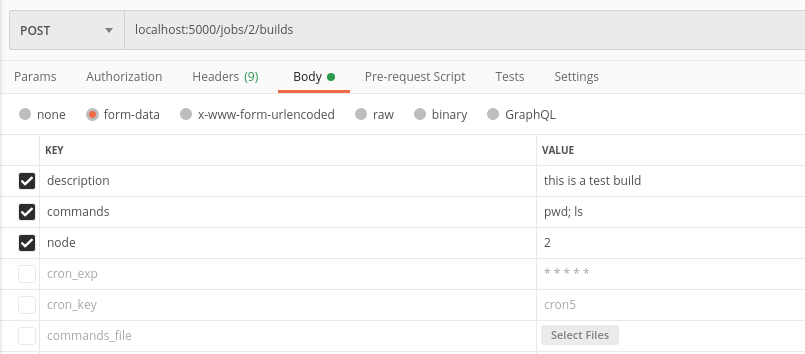
\includegraphics[scale=0.4]{postman_example2}
    \caption{HTTP POST example to be performed with Postman, self-elaboration}
\end{figure}

\newpage
\section{Results}

The results of this thesis basically consist on a REST API (the back-end) capable of automating jobs with CI and CD features and a basic client whose purpose is to ease the usage of the back-end. In the following table all the API entries are shown :

\begin{table}[H]
\centering
\begin{tabular}{|m{7cm}|m{1.6cm}|p{5cm}|}
\hline
\textbf{Route} & \textbf{Method} & \textbf{Description} \\ \hline
/jobs           & GET            & Returns a list of all the jobs    \\ \hline
/jobs           & POST            & Creates a job \newline \textbf{Params:} Title, Description    \\ \hline
/jobs/<int:job\_id>  & GET            & Returns a job with all info displayed  \\ \hline
/jobs/<int:job\_id>   & DELETE            &  Deletes a job    \\ \hline
/jobs/<int:job\_id>/builds    & GET            & Returns a list with all the builds contained on a job     \\ \hline
/jobs/<int:job\_id>/builds    & POST            &  Creates a build \newline \textbf{Params:} node, description, commands, cron\_exp, cron\_key, commands\_file \\ \hline
/jobs/<int:job\_id>/builds/<int:build\_id>           & GET            & Returns a build with all info displayed    \\ \hline
/jobs/<int:job\_id>/builds/<int:build\_id>           & DELETE            &  Deletes a build   \\ \hline
/nodes          & GET            &  Returns a list of all the nodes   \\ \hline
/nodes          & POST            & Creates a node \newline \textbf{Params:} workspace, ip\_addr, port, user, password    \\ \hline
/nodes/<int:node\_id>          & GET            &  Returns a node with all info displayed    \\ \hline
/nodes/<int:node\_id>          & DELETE            & Deletes a node     \\ \hline
/cron\_builds          & GET            &  Returns a list with all the Cron Builds stored in the db  \\ \hline
/cron\_build/<cron\_key>          & GET            &  Returns a Cron Build with all info displayed   \\ \hline
/cron\_build/<cron\_key>          & DELETE            & Deletes a Cron Build    \\ \hline

\end{tabular}
\caption{Back-end REST API documentation, source : Python docs}
\end{table}
\newpage

Regarding the front-end, routes are similar to the back-end but with slight differences, such as that there are specific routes for displaying the forms for job creation, build creation, etc.

\begin{table}[H]
\centering
\begin{tabular}{|m{7cm}|m{1.6cm}|p{5cm}|}
\hline
\textbf{Route} & \textbf{Method} & \textbf{Description} \\ \hline
/           & GET            & Displays the index page, showing the menu and nav bar    \\ \hline
/jobs           & GET            & Display the list of jobs    \\ \hline
/jobs           & POST            & Internal route called from creat\_job in order to perform an operation against the back-end    \\ \hline
/jobs/<int:job\_id>  & GET            & Displays the job info and all the builds contained in the job  \\ \hline
/jobs/<int:job\_id>  & POST            & Internal route called from creat\build in order to perform an operation against the back-end  \\ \hline
/jobs/<int:job\_id>/builds/<int:build\_id>           & GET            & Returns a build with all info displayed    \\ \hline
/nodes          & GET            &  Returns a list of all the nodes   \\ \hline
/create\_job          & GET            & Displays the job creation form  \\ \hline
/create\_build/<int:build\_id>         & GET            &  Displays the build creation form    \\ \hline


\end{tabular}
\caption{Front-end routes documentation, source : Python docs}
\end{table}

Some screenshots regarding above routes are attached in order to improve the comprehension of the routes :

\begin{figure}[H]
    \begin{minipage}{0.45\linewidth}
       
\includegraphics[width=\linewidth]{index}
        \caption{/}
    \end{minipage}
    \begin{minipage}{0.45\linewidth}
       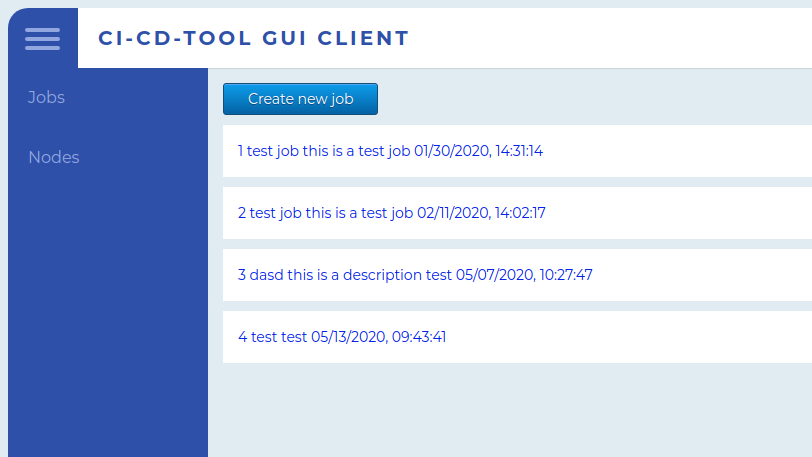
\includegraphics[width=\linewidth]{jobs}
        \caption{/jobs}
    \end{minipage}
\end{figure}

\begin{figure}[H]
    \centering
    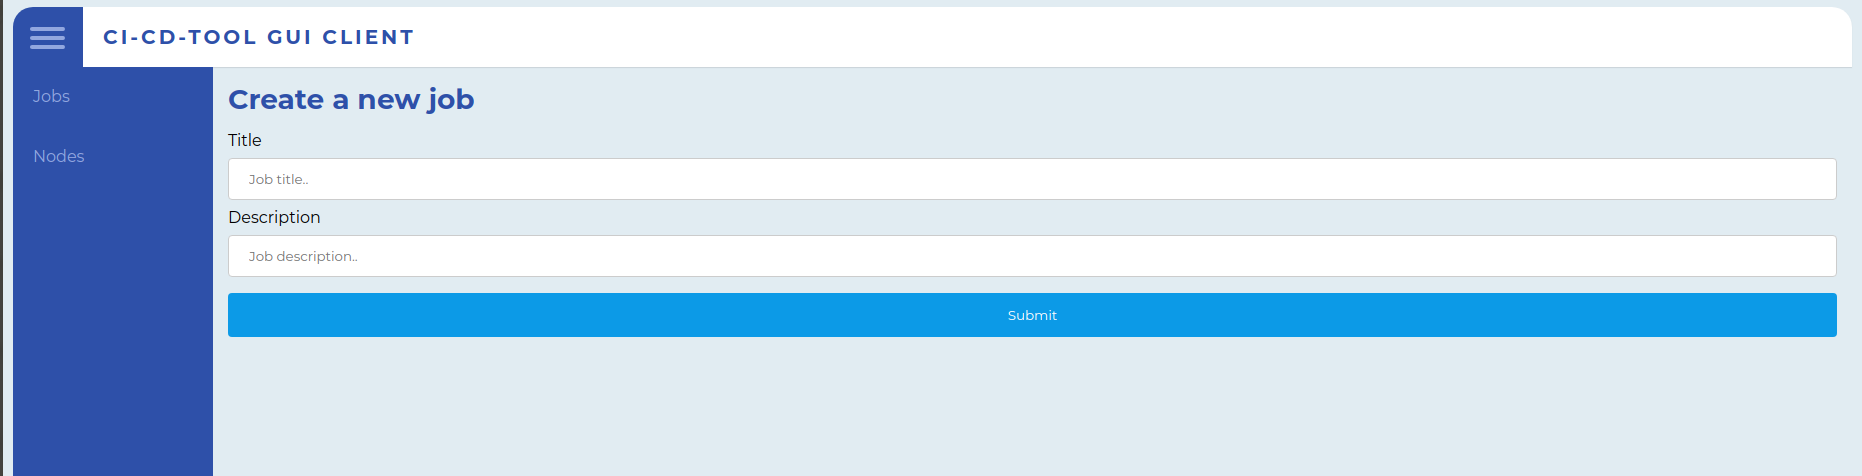
\includegraphics[scale=0.2]{create_job}
    \caption{/create\_job}
\end{figure}

\begin{figure}[H]
    \centering
    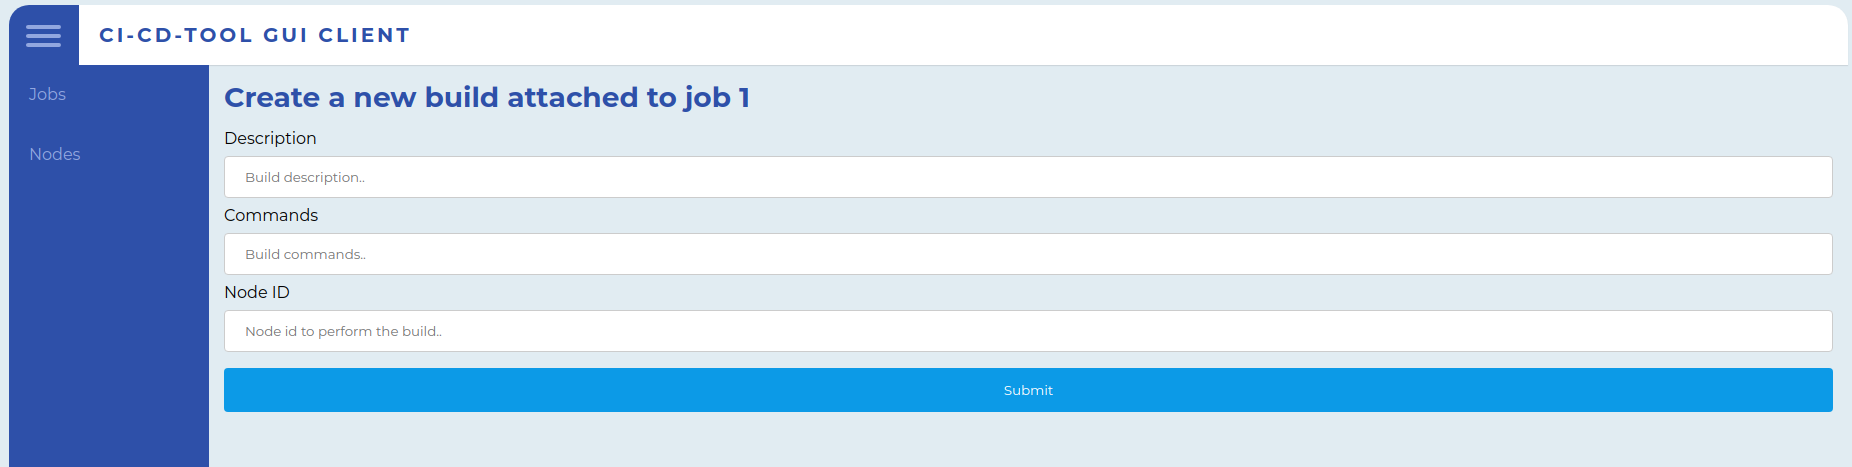
\includegraphics[scale=0.2]{create_build}
    \caption{/create\_build/<int:build\_id>}
\end{figure}

\subsection{Bringing up the tool}

In order to bring up the tool we have to start the back-end and the front-end WSGI bound to the ports desired, this is as easy as placing on the repository directory and execute gunicorn the following way using pipenv as explained before in detail:
~\\

\begin{lstlisting}
$ cd ci-cd-tool
$ pipenv shell
$ gunicorn -b localhost:5000  -w 4 src.app:app 
$ cd ../ci-cd-tool-client
$ pipenv shell
$ gunicorn -b localhost:8000  -w 4 app:app 
\end{lstlisting}

That way, we could access the client (front-end) by entering http://localhost:8000 URL on our browser, and we could perform calls to the REST API (back-end) to the localhost:5000 address.

\begin{lstlisting}

\end{lstlisting}

%EXAMPLE WITH SAMPLE PROJECT

\newpage
\section{Budget}

This project consisted mainly in two big tasks, research and development, hence the budget is adjusted to  the cost of these 2 activities, regarding licenses and tools used for the development I have only used Open Source and free community licenses.
~\\

The resulting costs based on above explanations are set by the amount of hours worked, 542 hours of dedication in total, setting a price per hour of 9 €/h which is the minimum stablished by the ETSETB for a degree student under a work agreement between a company and the university for 2019/2020 school season, the budget of this project is :
~\\

\begin{table}[H]
\centering
\begin{tabular}{|r|r|r|}
\hline
\textbf{Hours (h)} & \textbf{Price per hour (€/h)} & \textbf{Total (€)} \\ \hline
542                 & 9    & 4878 \\ \hline
\end{tabular}
\caption{Project budget}
\end{table}


\newpage
\section{Conclusions and future development}

DevOps is guiding companies through a transformation in the way of proceeding with software development and software delivery processes, this is the main reason why I wanted to get in touch first hand with this field in order to learn as much as possible about the culture. Regarding the general topic of the thesis, DevOps itself, it became very trending in the last decade and has a bright future granted along the lines of innovation and automation, due to the possibility of efficiently treating every project according to its own characteristics.
~\\

Designing a DevOps tool with CI and CD features has allowed me to directly get involved with a big part of the relevant concepts as well as strengthening my knowledge and thoughts on the topic and answering the questions I had before getting deeper on the research of this topic by comprehending the DevOps loop by putting it in practice with the tool.
~\\

This thesis aims to contribute on automating project tasks in what refers to CI and CD tasks, referring to the future development of the tool, as it will be used for some projects, different instances of the repository will be created with specific features required by each project, even though it is designed for being as much general as possible. Also, some general features are thought to be implemented in a future such as direct git and other tools integration, by using a \gls{DSL} (Domain Specific Language), which allows performing common operations such as working on the file-system or cloning repositories, etc, by using DSL commands on the pipelines. The goal of the tool is not to replace any other automation tool but to allow the parallel usage along with other services and reduce complexity, as this tool is easy to deploy and very lightweight.
~\\

On a personal note, the development of this thesis and my previous experience on the field has led me to focus my professional and labor career on DevOps, as it is a field where you can always learn new techniques of automation, new tools to work with, and there are also lot of events held annually regarding the topic in addition to the investment that big companies (such as Redhat or Amazon) and big open source projects (such as Docker or Kubernetes) are doing in order to stimulate, encourage and standardize the DevOps culture.
~\\

Researching and reading authors thoughts on the topic along these months have been very satisfying, I hope the reading of the thesis is also didactic for everyone who has not been introduced yet to DevOps culture, so you can get the basics on the topic and hopefully develop interest on the field, as I said before, there is a bright future on this field and companies are starting to compete for hiring DevOps engineers.

\newpage
\addcontentsline{toc}{section}{Bibliography}
\section*{Bibliography}
\nocite{*} % In order to print all entries
\printbibliography[heading=none]

\newpage
\addcontentsline{toc}{section}{Glossary}
\printglossaries

\end{document}
